\chapter{Related Work} \label{chapter:related_work}
In this section, we review related work on haptic output upon the face and examine previous works that use normal force to achieve haptic feedback.

\section{Haptic interaction in VR}
Simulated haptics is a key component to enhance immersion in virtual environments. Haptic interaction in VR has been extensively explored. Some works focused on installing the device on the limbs to generate partial haptic feedback for improving the realism in the virtual world, while others use large-scale device throughout the body to enhance feedback on immersive experiences.

\begin{figure}[h]
    \begin{center}
        \begin{tabular}{@{\hspace{0.1cm}}c}
           \includegraphics[width=1\textwidth]{figures/Hand_RelatedWork.pdf}
        \end{tabular}
        \captionof{figure}{(a) Haptic Revolver (b) 
Grabity}
        \label{fig:Hand_RelatedWork}
    \end{center}
\end{figure}

Most of the devices on the hand generating tactile feedback are mounted on the finger or palm. Whitmire et al. \cite{hapticrevolver} presented Haptic Revolver, a handheld VR controller that renders fingertip haptics when interacting with virtual surfaces. Grabity \cite{Grabity}, a wearable haptic device, demonstrated simulating grip forces and weight for grasping virtual objects in the virtual environment. In addition to tactile feedback for texture and precise finger manipulation, some other works focused on the bigger human motion on the arm and feet. Impacto \cite{Impacto} decomposed a series of the haptic sensation on limbs into tactile triggering and muscle contraction, using electrical muscle stimulation (EMS) embedded design to enhance the haptic feedback on limbs in VR. Lopes et al. \cite{VRwalls} actuated the user's shoulder, arm, and wrist muscles with EMS, creating a counter force that pulls the user's arm backward to add haptics to walls and other heavy objects in the virtual environment. Level-ups \cite{Level-up} showed a foot-mounted device with computer-controlled stilts that allows VR users to experience walking up and down steps.


\begin{figure}[h]
    \begin{center}
        \begin{tabular}{@{\hspace{0.1cm}}c}
           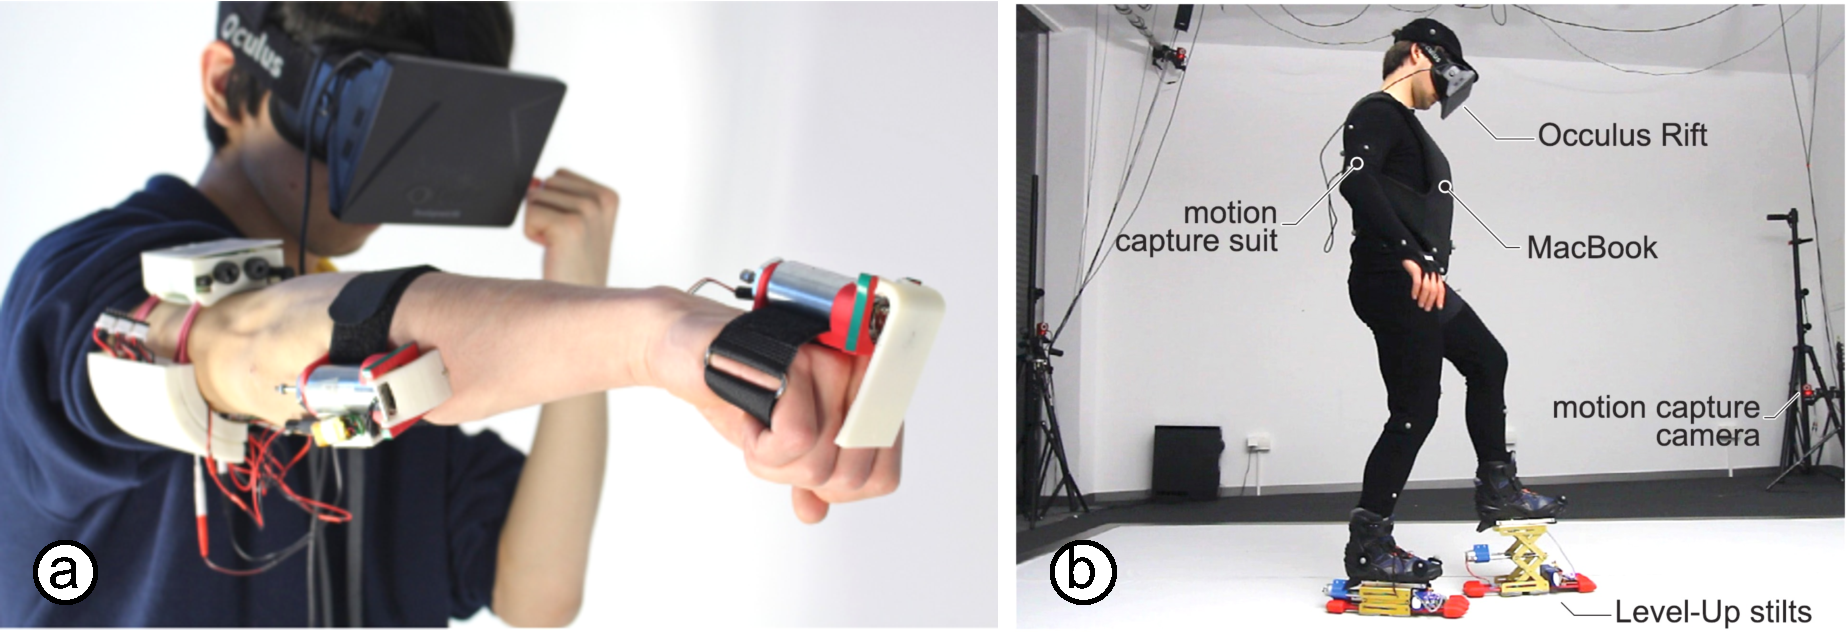
\includegraphics[width=1\textwidth]{figures/Force_RelatedWork.pdf}
        \end{tabular}
        \captionof{figure}{(a) Impacto (b) 
Levels-Up}
        \label{fig:Force_RelatedWork}
    \end{center}
\end{figure}

Apart from enhancing actuators on the human body, daily necessities have been adopted to enhance immersion. Gugenheimer et al. \cite{SwiVRChair} presented  SwiVRChair, which nudges users' orientation in 360-degree storytelling scenarios through a motorized swivel chair. Haptic Bed \cite{HapticBed} demonstrated a bed-style haptic display that provides weight sensation to the wide area of the user's body. Total resistance exercise (TRX) and elastic belts produce suspension force, enriching haptic force feedback. Hong et al. \cite{Wakeboarding} implemented Wakeboarding, in which the player riding a balance board in the reality skis on a meandering river in VR. The movement of the user was achieved by sustaining the weight and balance with the support of the suspension kit. Jain et al. \cite{Amphibian} created Amphibian, a simulator to simulate a wider variety of sensations experienced underwater through elastic band. Human-actuator also provides the user an immersive experience \cite{HapticTurk, TurkDeck}. Haptic Turk replaced motors and mechanical components with humans, a different approach to motion platforms that is light and mobile. TurkDeck produced the haptic sensation using props i.e. when users touch or manipulate an object in the virtual world, they simultaneously also touch or manipulate a corresponding object in the physical world. 


\section{Haptic Output on HMDs }
Although previous research has broadly explored various mechanisms generating different modes of haptic feedback in VR, many involved feedback as perceived via the limbs of the human body mainly achieved via handheld devices or wearable interfaces. Such haptic implementations on the limbs convey the concept of manipulating the virtual world directly. However, the human head is anatomically in charge of navigating and spatial awareness and can also be well-utilized to enhance a sense of immersion during VR encounters. The mere action of channeling haptic feedback directly through an HMDs acts as a directional information-containing medium and its design is also challenging due to the fact that every device has to be integrated into an overarching system.

\begin{figure}[h]
    \begin{center}
        \begin{tabular}{@{\hspace{0.1cm}}c}
           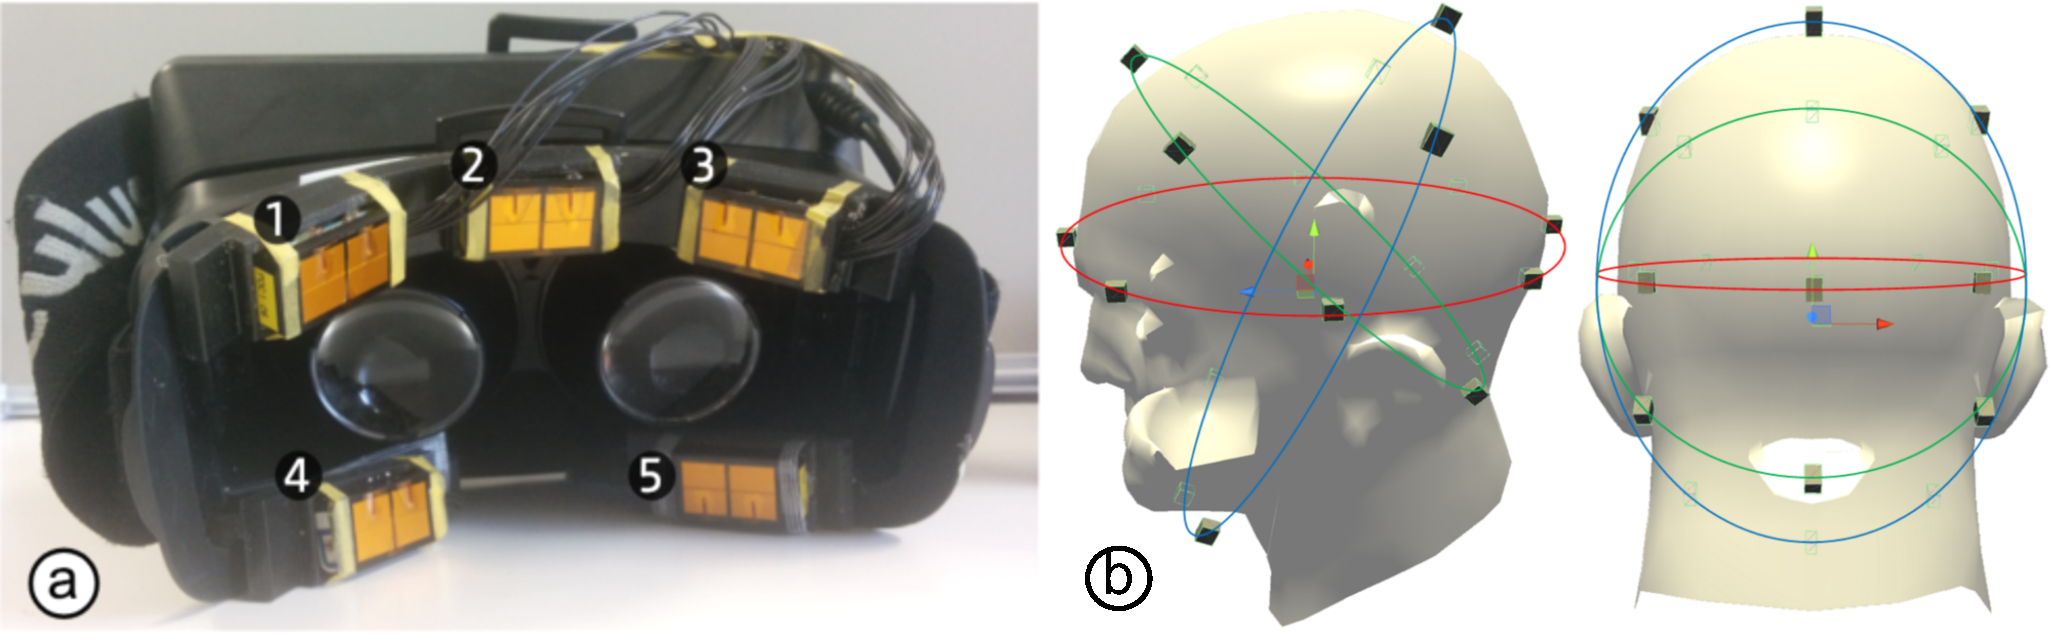
\includegraphics[width=1\textwidth]		{figures/Head_RelatedWork.pdf}
        \end{tabular}
        \captionof{figure}{(a) ThermoVR (b) 
HapticHead}
        \label{fig:Head_RelatedWork}
    \end{center}
\end{figure}

In prior research works vibrotactile feedback is implemented via HMDs that transforms haptic output into directional and guidance cues in a 3D space \cite{VibGuide, HapticHead, Vibroplay}. Consequently a vibrotactile device can be installed inside the contact region of an HMD directly and exploited as a navigation indicator \cite{VibGuide}. HapticHead \cite{HapticHead} distributes multiple vibrotactile actuators in three concentric ellipses around the head to provide intuitive haptic guidance. Vibroplay \cite{Vibroplay} extended the functionality of vibrotactile output in VR into a direct authoring manipulation system. In addition to vibrotactile feedback, thermal may be utilized as another haptic output component in a virtual environment. ThermoVR \cite{ThermoVR} demonstrates embedding of five thermal modules via HMD, which produce hot and cold haptic feedback. The different locations of thermal stimuli had been used prior as a directional cue in exploring the virtual world. Ranasinghe, et al., \cite{Ambiotherm} implements Ambiotherm, a multimodal interface including temperature modules attached to the neck and wind modules attached to the HMD allowing users to experience the sensation of wind on her/his face and the feeling of heat on the skin. 

\begin{figure}[h]
    \begin{center}
        \begin{tabular}{@{\hspace{0.1cm}}c}
           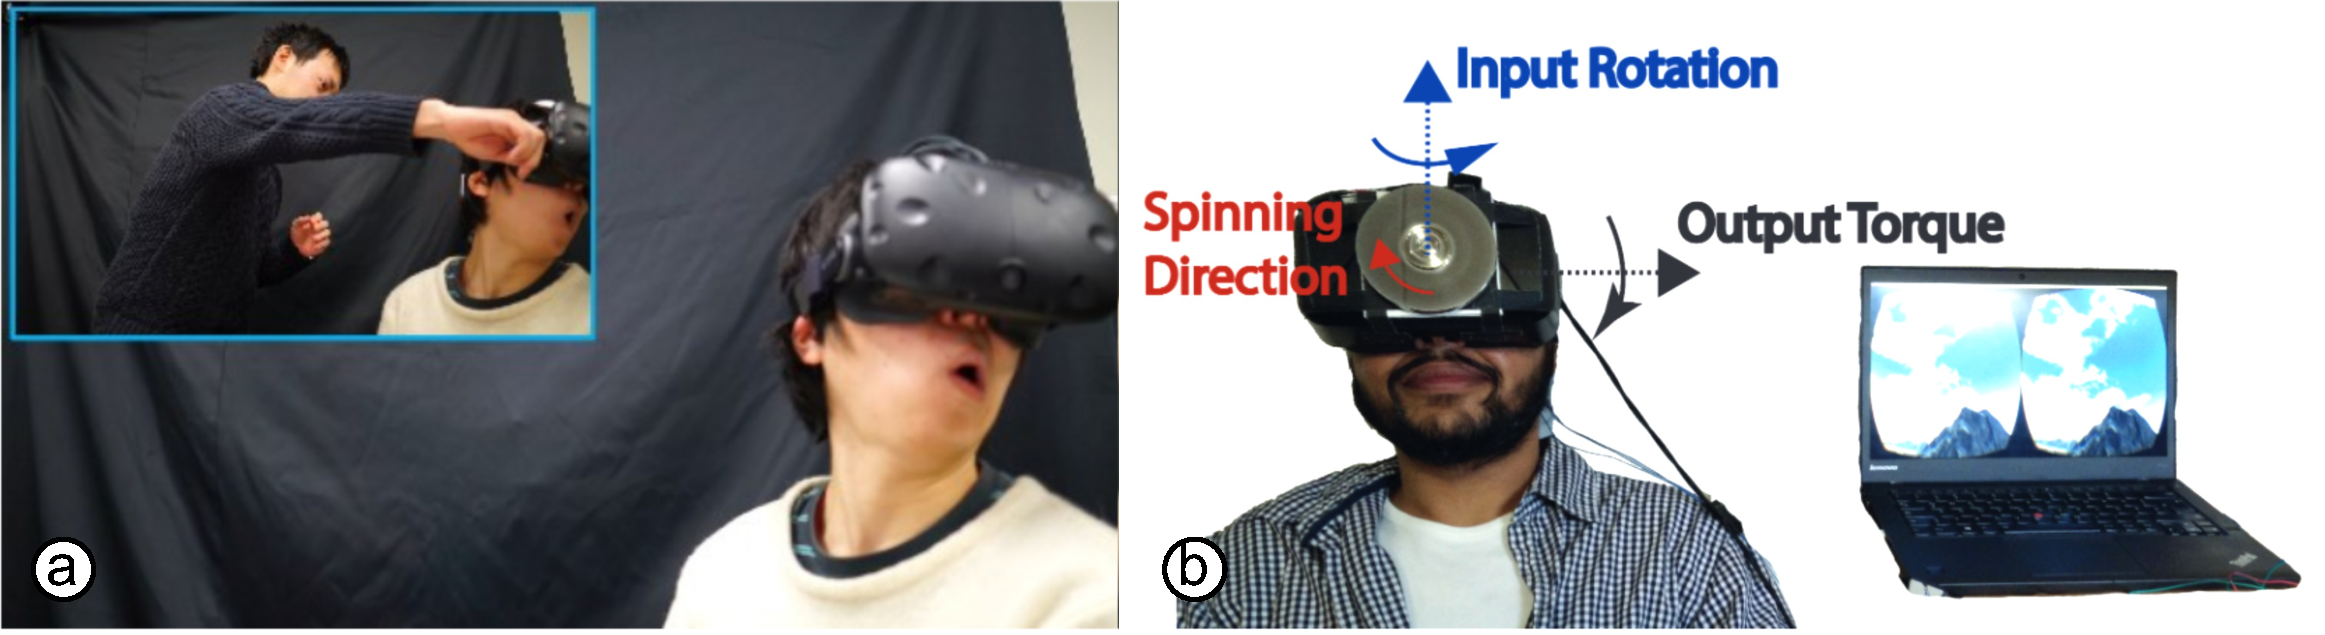
\includegraphics[width=1\textwidth]		{figures/HeadForce_RelatedWork.pdf}
        \end{tabular}
        \captionof{figure}{(a) HangerOVER (b) 
GyroVR}
        \label{fig:HeadForce_RelatedWork}
    \end{center}
\end{figure}

Other works focus on simulating head movements through force feedback. GyroVR \cite{GyroVR} contains a gyroscope attached to the HMD generating tangential force, which provides a feeling of inertia when conveying fast motion or an altered environment in VR. Sato, et al., \cite{hangerreflex09} introduce a phenomenon called “Hanger Reflex” and utilize its mechanism to implement a head rotation interface through a hanger. Kon, et al. \cite{hangerreflex16} extended the hanger reflex interface into a wearable haptic device, which can be installed on the waist. HangerOver \cite{HangerOVER} demonstrates a hanger reflex system incorporated into the HMD, allowing simulation of being pushed or punched enhancing rotation movement in a virtual environment \cite{HangerOVER}. Aoyama, et al., \cite{GVS} present the Electrode that can also simulate virtual head movement which uses galvanic vestibular stimulation (GVS) to induce a feeling of directional virtual head motion through four electrodes. Finally, GVS Ride \cite{GVSRIDE} demonstrates tri-directional acceleration through a four-pole GVS mounted with HMD.

\section{Normal Force as a Haptic Output }

\begin{figure}[h]
    \begin{center}
        \begin{tabular}{@{\hspace{0.1cm}}c}
           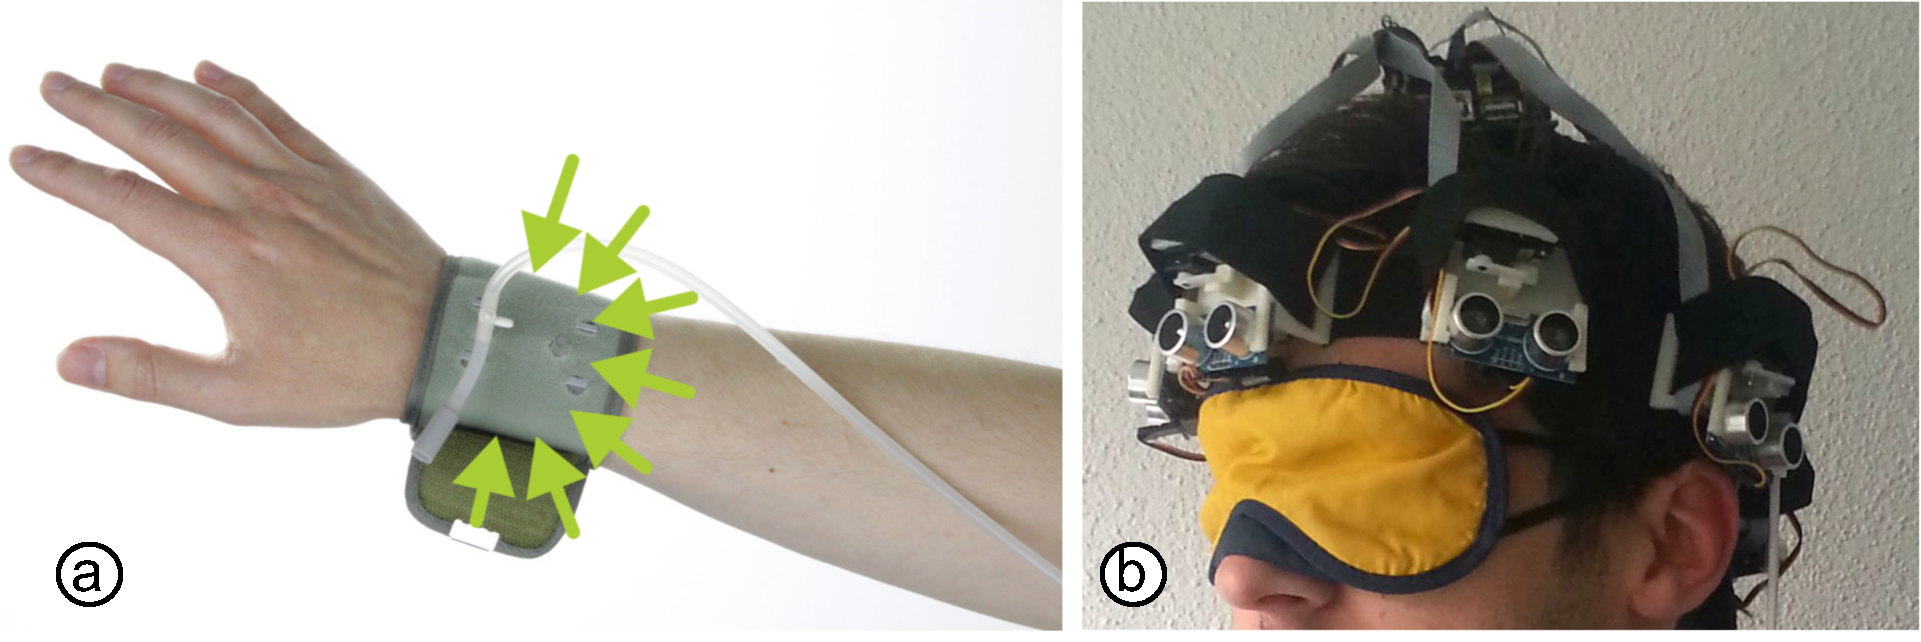
\includegraphics[width=1\textwidth]		{figures/NormalForce_RelatedWork1.pdf}
        \end{tabular}
        \captionof{figure}{(a) Squeezeback (b) 
ProximityHat}
        \label{fig:NormalForce_RelatedWork1}
    \end{center}
\end{figure}

Human beings experience normal force on a certain skin surface as a sensation of pressure through mechanoreceptors. Squeezeback \cite{Squeezback} presents the use of pneumatic actuation and inflatable straps to create compression stimulus on the wrist for notification. HapticClench \cite{HapticClench} demonstrates a squeezing sensation with a shape memory alloy on the wrist. Delazio, et al., \cite{forceJacket} presents Force Jacket, a wearable jacket attached with pneumatically actuated airbags and force sensors that provide precisely directed force and high frequency vibrations to the upper body. Berning, et al., \cite{ProximityHat} implement ProximityHat which consists of wearable pressure actuators placed around the head to convey spatial information. Based on these previous works just mentioned, we deploy the spatial information concept through FacePush which generates normal force feedback on a horizontal axis of the face via the HMD.

\begin{figure}[h]
    \begin{center}
        \begin{tabular}{@{\hspace{0.1cm}}c}
           \includegraphics[width=1\textwidth]		{figures/NormalForce_RelatedWork2.pdf}
        \end{tabular}
        \captionof{figure}{(a) HapticClench (b) 
Force Jacket}
        \label{fig:NormalForce_RelatedWork2}
    \end{center}
\end{figure}
